\section{Ход работы}

Пусть имеются база данных с таблицами store и manufacturers (рисунки 3.1-3.3).

\begin{figure}[h!t]
    \center{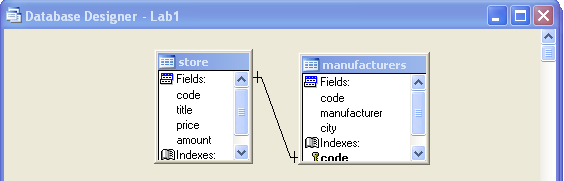
\includegraphics[width=0.7\linewidth]{structure}}
  \caption{Схема базы данных}
\end{figure}

\begin{figure}[h!t]
    \center{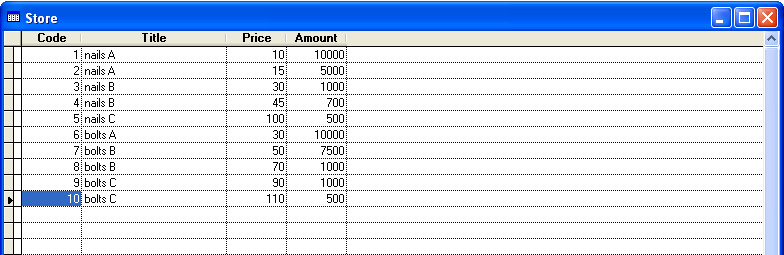
\includegraphics[width=1\linewidth]{store}}
  \caption{Содержимое таблицы Store}
\end{figure}

\begin{figure}[h!t]
    \center{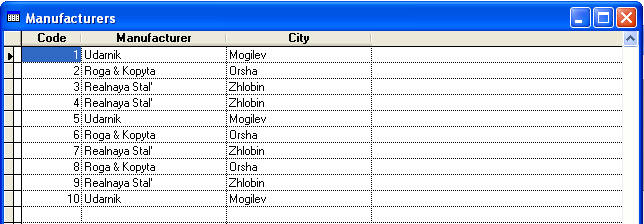
\includegraphics[width=1\linewidth]{manufacturers}}
  \caption{Содержимое таблицы Manufacturers}
\end{figure}

\pagebreak

Создадим визуальный класс для реализации парадигмы CRUD.

\begin{figure}[ht]
    \center{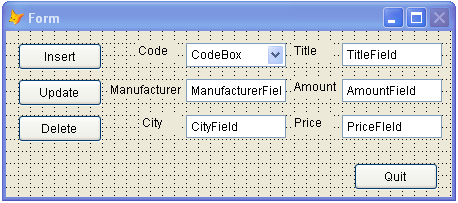
\includegraphics[width=0.7\linewidth]{class}}
  \caption{Форма класса myForm}
\end{figure}

Ниже приведены листинги используемых методов класса.

\begin{lstlisting}[float=h,caption=myForm.getData]
  curCode = VAL(thisForm.codeBox.Value)

  SELECT * FROM store INNER JOIN manufacturers ON store.code=manufacturers.code WHERE store.code = curCode INTO CURSOR dataCursor

  thisForm.manufacturerField.Value = dataCursor.manufacturer
  thisForm.cityField.Value = dataCursor.city

  thisForm.titleField.Value = dataCursor.title
  thisForm.priceField.Value = dataCursor.price
  thisForm.amountField.Value = dataCursor.amount
\end{lstlisting}

\begin{lstlisting}[float=h,caption=myForm.insertData]
  SELECT MAX(code) FROM store INTO CURSOR availableCode
  newCode = availableCode.max_code
  newTitle = thisForm.titleField.value
  newPrice = thisForm.priceField.value
  newAmount = thisForm.amountField.value
  newManufacturer = thisForm.manufacturerField.value
  newCity = thisForm.cityField.value

  INSERT INTO store values(newCode + 1, newTitle, newPrice, newAmount)
  INSERT INTO manufacturers values(newCode + 1, newManufacturer, newCity)
\end{lstlisting}

\begin{lstlisting}[float=h,caption=myForm.updateData]
  curCode = VAL(thisForm.codeBox.value)
  newTitle = thisForm.titleField.value
  newPrice = thisForm.priceField.value
  newAmount = thisForm.amountField.value
  newManufacturer = thisForm.manufacturerField.value
  newCity = thisForm.cityField.value

  UPDATE store SET title = newTitle WHERE code = curCode
  UPDATE store SET price = newPrice WHERE code = curCode
  UPDATE store SET amount = newAmount WHERE code = curCode
  UPDATE manufacturers SET manufacturer = newManufacturer WHERE code = curCode
  UPDATE manufacturers SET city = newCity WHERE code = curCode
\end{lstlisting}

\begin{lstlisting}[float=h,caption=myForm.deleteData]
curCode = VAL(thisForm.codeBox.value)

DELETE FROM store WHERE (code = curCode)
SELECT store
DELETE FROM manufacturers WHERE (code = curCode)
SELECT manufacturers
\end{lstlisting}

\begin{lstlisting}[float=h,caption=myForm.getAvailableCode]
  LPARAMETERS eFormat, aData

  SELECT code FROM store INTO CURSOR availableCode
  WITH thisForm.codeBox
	.rowSource = 'availableCode.code'
	.rowSourceType = 2
	.boundColumn = 1
	.boundTo = .t.
	.Style = 2
	.ListIndex = 1
  ENDWITH
\end{lstlisting}

\begin{lstlisting}[float=h,caption=InsertButton.Click]
  thisForm.insertData
  thisForm.getavailablecode
\end{lstlisting}

\begin{lstlisting}[float=h,caption=UpdateButton.Click]
  thisForm.updatedata
\end{lstlisting}

\begin{lstlisting}[float=h,caption=DeleteButton.Click]
  thisForm.deleteData
  thisForm.getavailablecode
  thisForm.getData
\end{lstlisting}

\begin{lstlisting}[float=h,caption=CodeBox.Click]
  thisForm.getData
\end{lstlisting}

\begin{lstlisting}[float=h,caption=CodeBox.Init]
  thisForm.getavailablecode
\end{lstlisting}

\begin{lstlisting}[float=h,caption=CodeBox.Init]
  thisForm.Release
\end{lstlisting}

\begin{lstlisting}[float=h,caption=runCRUD]
PROCEDURE runCRUD
	SET CLASSLIB TO "\\hp\budnyjj\university\labs\bibd\lab_3\class\myform.vcx" ADDITIVE
	myForm = CREATEOBJECT("myform")
	myForm.Show
	READ EVENTS
	RETURN
ENDPROC
\end{lstlisting}